\chapter{Comparative Genomic Analysis of \emph{P. papatasi} and \emph{L. longipalpis} Sand Fly Genomes}

\section{Introduction}
Leishmaniasis is a disease caused by protozoan parasites. Leishmaniasis occurs in multiple forms. Cutaneous leishmaniasis infects the skin, causing painful sores which can reoccur up to 20 years after infection, even in individuals who have been adequately treated. The deadly form visceral leishmaniasis is the second-largest parasitic killer in the world, responsible for 200,000 to 400,000 infections per year worldwide; the largest being malaria.

The protozoans responsible for Leishmaniasis are transmitted by phlebotomine sand flies, diverse group of vectors that vary widely in geographic distribution, ecology, and the pathogens they transmit. \emph{Phlebotomus papatasi}, found in the Old World (particularly, Northern Africa and the Middle East), is the major vector of cutaneous leishmaniasis, while \emph{Lutzomyia longipalpis} is the main vector of visceral leishmaniasis in Latin America, where it is found.

The genomes of \emph{P. papatasi} and \emph{L. longipalpis} have recently been sequenced, with the goal of furthering population control efforts. Such efforts are not without precedent. Simiar genomic analysis of Anopheles mosquito malaria vectors has resulted in the identification of new species as well as genes associated with variations in insecticide resistance, leading to improvements in  population control efforts.

\emph{L. longipalpis} is a complex of sibling species, previously identified through analyses of copulation songs, sex pheromones and molecular markers.  Analyses of population genetics through whole-genome sequences could answer questions such about the exact number of species, the level of divergence, and gene flow.  Of particular interest are how the subspecies may differ in insecticide resistance and immune response to the Leishmaniasis protozoan parasites.

Similar questions surround \emph{P. papatasi}.  Previous analyses of microsatellites of 188 \emph{P. papatasi} individuals from 35 sites in 15 countries indicates two distinct populations, A and B.  Population A contained five subpopulations whose genetic differences correlated with differences in geographical origin of the individuals.  Population B consisted of individuals collected in the Middle East and northern Mediterranean area but genetic differences in subpopulations lacked correlation with geographical origin.

Here, we focus on a genomic comparison of \emph{P. papatasi} and \emph{L. longipalpis}, using the mosquitoes \emph{Ae. aegypti} and \emph{An. gambiae} and fruit flies \emph{D. melanogaster} and \emph{D. simulans} as controls.  We begin by analyzing completeness of the sand fly genome assemblies, finding that the assemblies are quite fragmented.  We follow with analysis of synteny, finding multiple microsynteny blocks between \emph{P. papatasi} and \emph{L. longipalpis} and \emph{P. papatasi}, \emph{L. longipalpis}, and \emph{An. gambiae}. Analyses of dN/dS, the rate of non-silent substitutions to silent substitutions, distributions for single-copy orthologs indicate no major surprises.  Lastly, we look at differential gene expression in blood-fed, sugar-fed, and infected blood-fed individuals of \emph{P. papatasi} using RNASeq, focusing on gene families associated with immune response.

\section{Methods}

\subsection{Data sets}
The \emph{Ae. aegypti}, \emph{An. gambiae}, \emph{L. longipalpis}, and \emph{P. papatasi} \textcolor{red}{TODO VERSIONS} peptide translations were downloaded from Vectorbase \textcolor{red}{TODO CITE}, while the \emph{D. melanogaster} and \emph{D. simulans} peptide translations were downloaded from Flybase \textcolor{red}{TODO CITE}.

\textcolor{red}{table of versions and sources}

\subsection{Assembly Statistics}
Cumulative density function plots of the gene distributions over the scaffolds were generated as follows: The gene counts of each genome's scaffolds were normalized by dividing the gene counts by the number of genes in that organism's genome. For each genome, lists of the normalized gene counts were sorted largest to smallest and padded with 0-value entries so that all of the lists had the same length.  Cumulative sums were computed over the normalized gene counts and plotted.


\subsection{Synteny}
To generate the scatter plots, the identifiers, scaffolds, locations, and sense in the FASTA headers were extracted for each peptide sequence.  The protein IDs were cross-referenced with OrthoDB to group the proteins into ortholog groups.  Sequences without ortholog information or no orthologs in the other genomes and ortholog groups with many-to-many and one-to-many relationships were discarded.  The proteins were sorted along each scaffold by their starting coordinates, while scaffolds were ordered arbitrarily.  Scatter plots were generated by drawing dots at the positions of orthologous proteins.

Microsynteny blocks were identified using SynChro. For each genome, the identifiers, protein sequences, orientations, scaffolds, and locations extracted from FASTA files for each genome and reformatted as input for CHROnicle and SynChro \textcolor{red}{TODO CITE}.  SynChro ($\Delta=5$) was run on the pairs \emph{D. melanogaster} and \emph{D. simulans}, \emph{An. gambiae} and \emph{L. longipalpis}, \emph{An. gambiae} and \emph{Ae. aegypti}, and \emph{L. longipalpis} and \emph{P. papatasi}.  Three-way synteny blocks for \emph{An. gambiae}, \emph{L. longipalpis}, and \emph{P. papatasi} were constructed by finding all pairs of synteny blocks for \emph{An. gambiae} and \emph{L. longipalpis} and \emph{L. longipalpis} and \emph{P. papatasi} that overlapped by at least one gene.  

The top five largest (by counts of total genes) synteny blocks from selected from the \emph{L. longipalpis} and \emph{P. papatasi} and \emph{Ae. aegypti}, \emph{L. longipalpis}, and \emph{P. papatasi} comparisons.  Genes were annotated using BLAST against the NCBI database.

\subsection{dN/dS Distributions}
Selective constraints on gene sequence evolution were estimated using the dN/dS statistic calculated for orthologous group multiple sequence alignments. Protein sequences were organized into ortholog groups according to OrthoDB v8 \textcolor{red}{TODO CITE}. Groups that did not have at least one sequence from each species were discarded.  For groups with 1-to-many and many-to-many orthologs, one protein sequence was chosen randomly from each species with uniform weights. Protein multiple sequence alignments were generated using Clustal Omega \textcolor{red}{TODO CITE} and used to inform CDS alignments with the codon-aware PAL2NAL alignment program \textcolor{red}{TODO CITE}.  The yn00 program from PAML v4.8 \textcolor{red}{TODO CITE} was used to calculate dN/dS ratios for each pairs of sequences in the aligned ortholog groups.

\subsection{RNASeq}

\textcolor{red}{TODO Cuffdiff}

Gene identifiers for genes marked as statistically significant by \texttt{CuffDiff} were extracted for each time point and feeding condition.  The corresponding protein sequences for each gene were extracted from the genomes.  The protein sequences were merged and run through \texttt{BLAST2GO}. \textcolor{red}{TODO CITE, VERSION}

\section{Results}

\subsection{Analysis of Genome Assembly Fragmentation}
Fragmentation of a genome assembly significantly effects comparative genomic analysis.  In particular, if the assembly produces a large number of scaffolds with only or two genes that cannot be mapped back to chromosomes, analyses such as synteny will not produce interpretable results.  To place our analyses discussed below in context, we analyzed the amount of fragmentation occurring in the sand fly genomes.  We our analysis found evidence of significant fragmentation.

\textcolor{red}{why the choices of species?}

We analyzed and compared the distribution of genes across the scaffolds from the genomes of the sand flies \emph{Ph. papatasi} and \emph{Lu. longipalpis}, mosquitoes \emph{Ae. aegypti} and \emph{An. gambiae}, and fruit flies \emph{Dr. melonagaster} and \emph{Dr. simulans} (Figure~\ref{fig:scaffolds}).  The six organisms have between 10,100 and 17,294 genes.  Assemblies of the \emph{An. gambiae} and \emph{Dr. melonagaster} genomes are relatively complete and are used as our standard for comparison.  \emph{An. gambiae} and \emph{Dr. melonagaster} both have one scaffold per chromosome with between 1,000 and 4,000 genes located on the five largest scaffolds.

The assembly of the \emph{Dr. simulans} genome is partially fragmented but still relatively complete.  The assembly has more scaffolds (1,131) than chromosomes, but sizes (in terms of genes) of the five largest scaffolds are comparable to \emph{An. gambiae} and \emph{Dr. melonagaster}.  Comparison of the cumulative distribution of gene locations from largest to smallest scaffolds suggests that a majority of \emph{Dr. simulans}'s genes are located on a small number of large scaffolds with about 10\% of the genes distributed across a number of small scaffolds.

Analysis of \emph{Ph. papatasi}, \emph{Lu. longipalpis}, and \emph{Ae. aegypti} suggest a different story, with high levels of fragmentation.  \emph{Ph. papatasi} has more than 4,300 scaffolds.  Fewer than 100 genes are located on each of the top five largest scaffolds of all three organisms.  The cumulative distribution of genes indicates that the genes of \emph{Ph. papatasi} are nearly uniformly distributed across the scaffolds.  while the genes of \emph{Lu. longipalpis} and \emph{Ae. aegypti} are mostly concentrated among a smaller number of scaffolds, more than 10\% of the genes appear to be distributed across a large number of small scaffolds.

\begin{figure}[H]
  \centering
  \begin{subfigure}[b]{0.45\textwidth}
    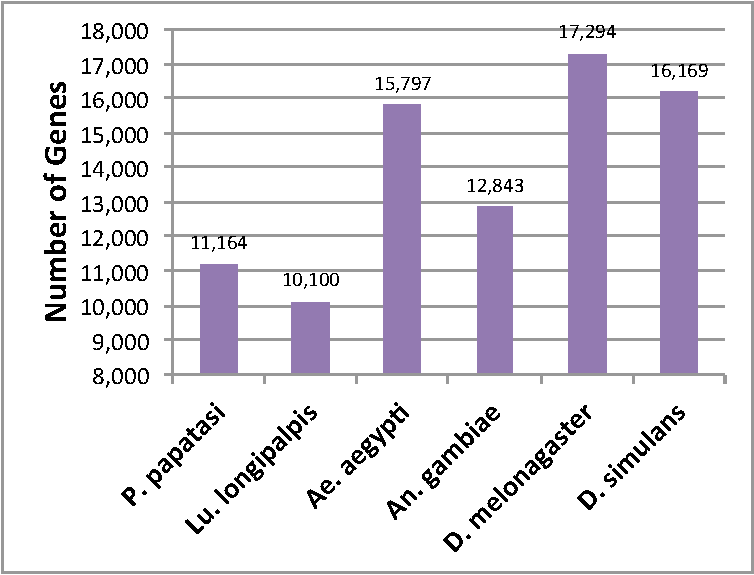
\includegraphics[width=\textwidth]{figures/synteny/genome_size_genes.pdf}
    \caption{Genome Sizes (Genes)}
  \end{subfigure}
  ~
  \begin{subfigure}[b]{0.45\textwidth}
    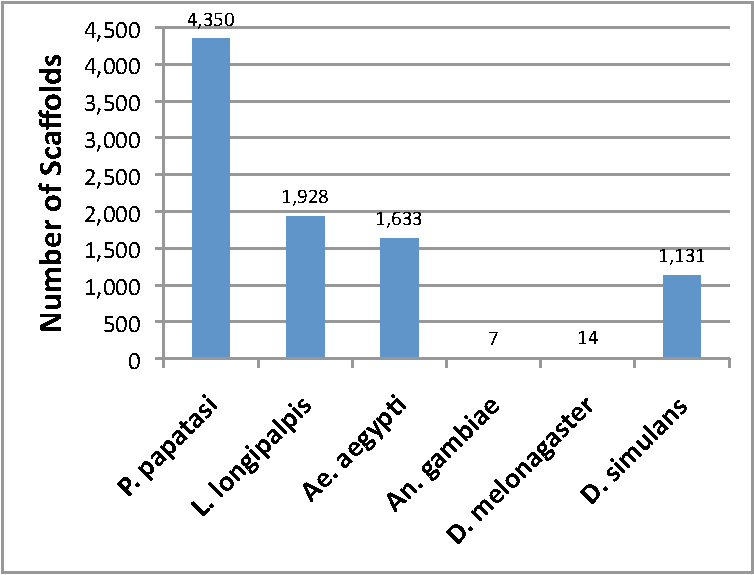
\includegraphics[width=\textwidth]{figures/synteny/scaffold_counts.pdf}
    \caption{Number of Scaffolds}
    \label{fig:number-scaffolds}
  \end{subfigure}
  ~
  \begin{subfigure}[b]{0.45\textwidth}
    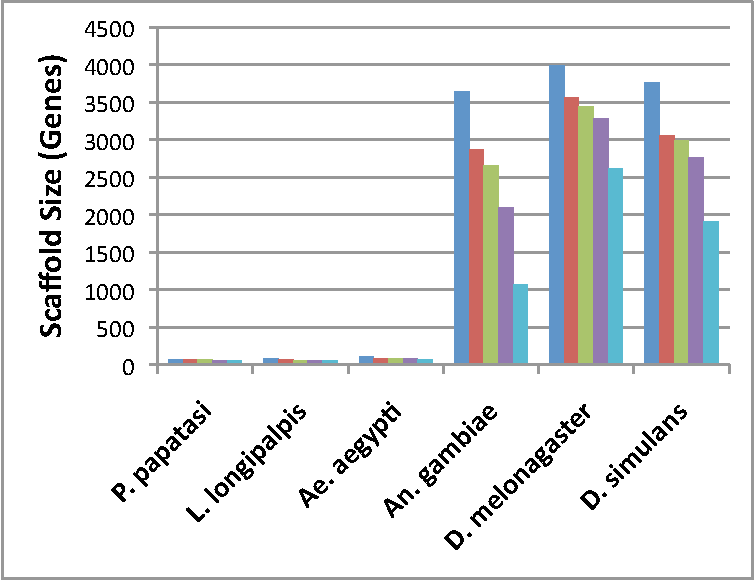
\includegraphics[width=\textwidth]{figures/synteny/top5_scaffold_sizes.pdf}
    \caption{Top 5 Scaffold Sizes (Genes)}
  \end{subfigure}
  ~
  \begin{subfigure}[b]{0.45\textwidth}
    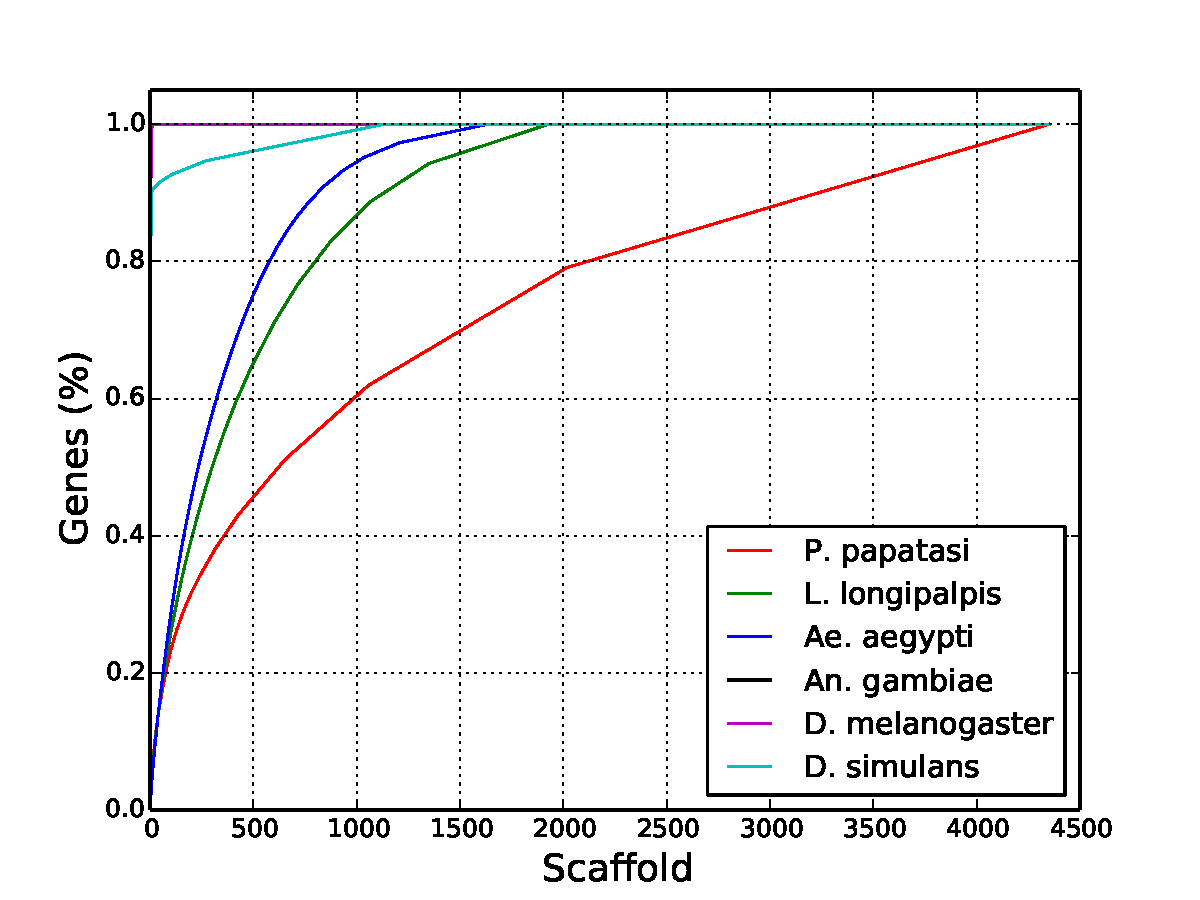
\includegraphics[width=\textwidth]{figures/synteny/gene_scaffold_cdf.pdf}
    \caption{Scaffold Genes CDF}
  \end{subfigure}
  \caption{}
  \label{fig:scaffolds}
\end{figure}

\subsection{Qualitative Analysis of Synteny}
Rearrangements of chromosomes are rare events and tend to happen in a block-wise fashion that mainly preserves the local order of genes on the chromosome. Thus, even after long periods of divergence between species, synteny blocks, defined as conserved runs of consecutive orthologous genes, remain discernible \cite{Heger2007}.  The presence of synteny can be used to infer evolutionary relationships between organisms' genomes at a macroscopic level, complementing analyses such as gene family expansions and reductions and changes within pairs of orthologous genes \cite{Zdobnov2002,Zdobnov2007}.

Synteny between pairs of dipterans was analyzed qualitatively by generating scatter plots where each axis represents genes locations for one species and dots are drawn where orthologs occur (see Section~\ref{sec:synteny-methods-dotplots}). The presence of significant synteny was not detectable between any pair of \emph{An. gambiae}, \emph{D. melanogaster}, \emph{L. longipalpis}, and \emph{P. papatasi} (Figure~\ref{fig:synteny-dotplots-sandflies}).  In contrast, we compared the synteny between \emph{D. melanogaster} and \emph{D. simulans} (Figure~\ref{fig:synteny-dotplots-drosophila}) as a control and found significant presence of synteny, including an inversion.

We followed up the qualitative analysis up with a quantitative analysis of synteny blocks computed using the program SynChro (see Section~\ref{sec:synteny-methods-synchro}). As indicated by the qualitative analysis, synteny was most conserved between \emph{D. melanogaster} and \emph{D. simulans} (243 synteny blocks with the largest block size of 700 genes, an average size of 41.6 genes, and a median size of 5 genes).  When compared to each other or \emph{An. gambiae}, the sand flies exhibited little conservation of synteny with the largest blocks consisting of far fewer genes than those from \emph{D. melanogaster} and \emph{D. simulans} (24 genes from \emph{L. longipalpis} and \emph{P. papatasi}, 39 genes from \emph{L. longipalpis} vs. \emph{An. gambiae}, and 21 genes from \emph{P. papatasi} vs. \emph{An. gambiae}).

We annotated and analyzed the largest synteny blocks from \emph{L. longipalpis} and \emph{P. papatasi}. and a three-way comparison of \emph{An. gambiae}, \emph{L. longipalpis}, and \emph{P. papatasi}.  Four of the largest synteny blocks from \emph{L. longipalpis} and \emph{P. papatasi} contained peritrophin-like, membrane-bound or -associated, RNA regulation and synthesis, and intracellular processes genes. \textcolor{red}{three-way comparison}

\begin{figure}[H]
  \centering
  \begin{subfigure}[b]{0.45\textwidth}
    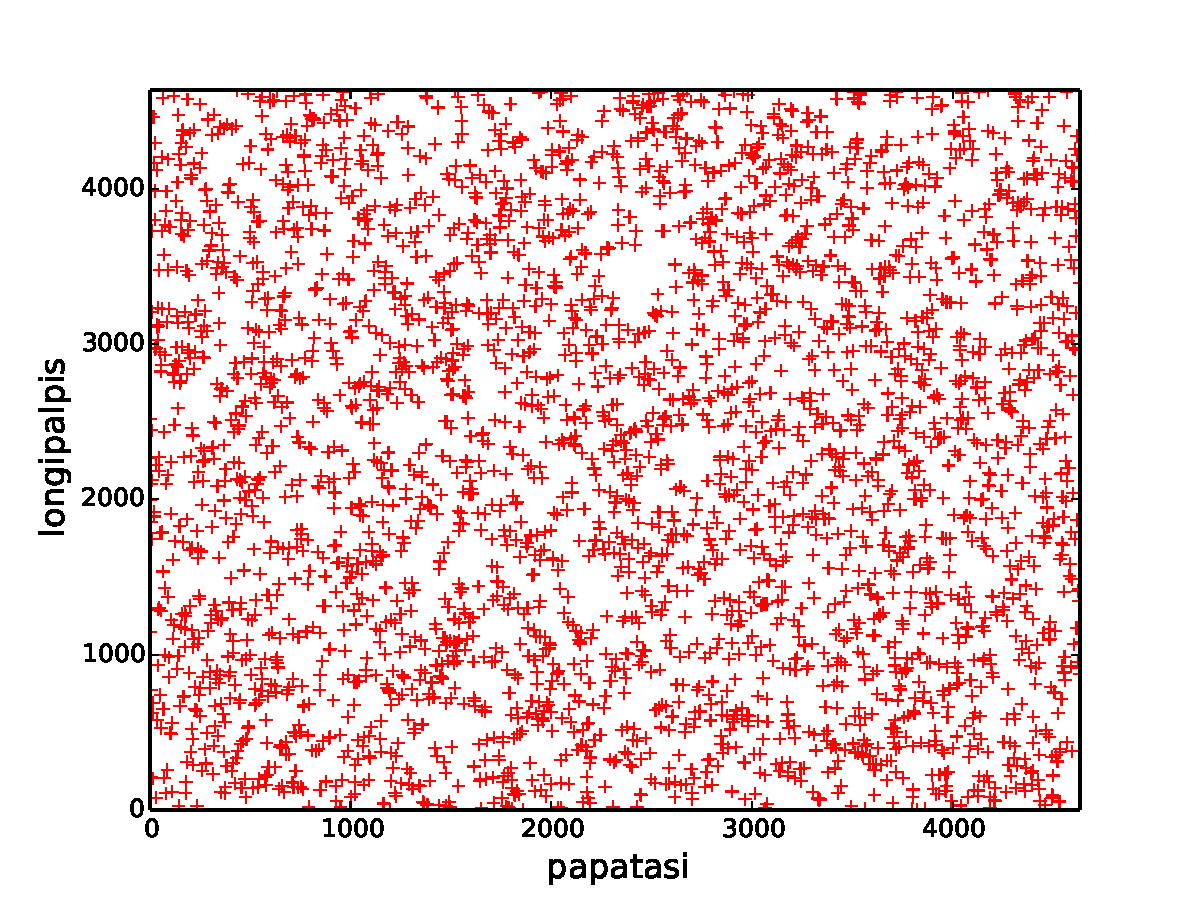
\includegraphics[width=\textwidth]{figures/synteny/papatasi_longipalpis_plot}
    \caption{\emph{L. longipalpis} vs. \emph{P. papatasi}}
    \label{fig:synteny-dotplots-sandflies}
  \end{subfigure}
  \\
  \begin{subfigure}[b]{0.45\textwidth}
    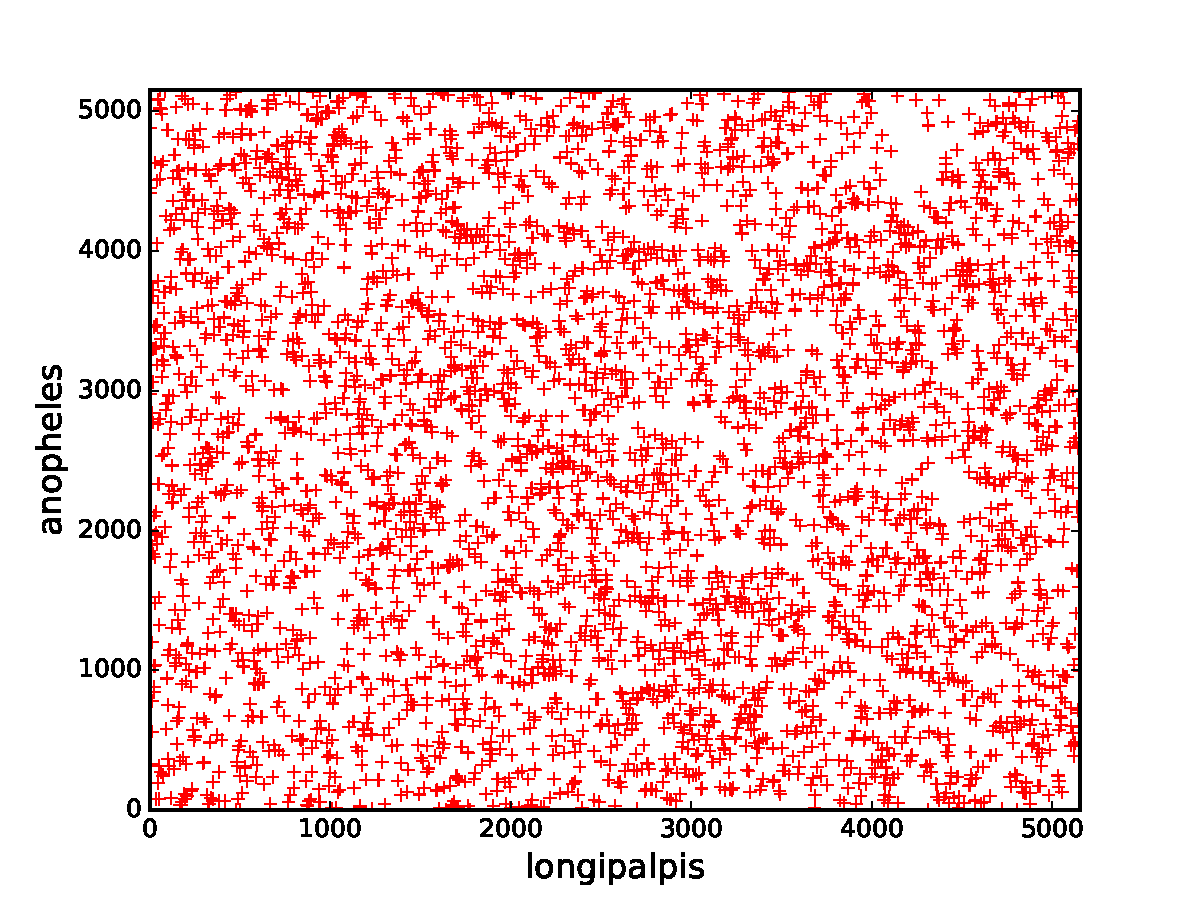
\includegraphics[width=\textwidth]{figures/synteny/longipalpis_anopheles_plot}
    \caption{\emph{L. longipalpis} vs. \emph{An. gambiae}}
    \label{fig:synteny-dotplots-longipalpis-anopheles}
  \end{subfigure}
  ~
  \begin{subfigure}[b]{0.45\textwidth}
    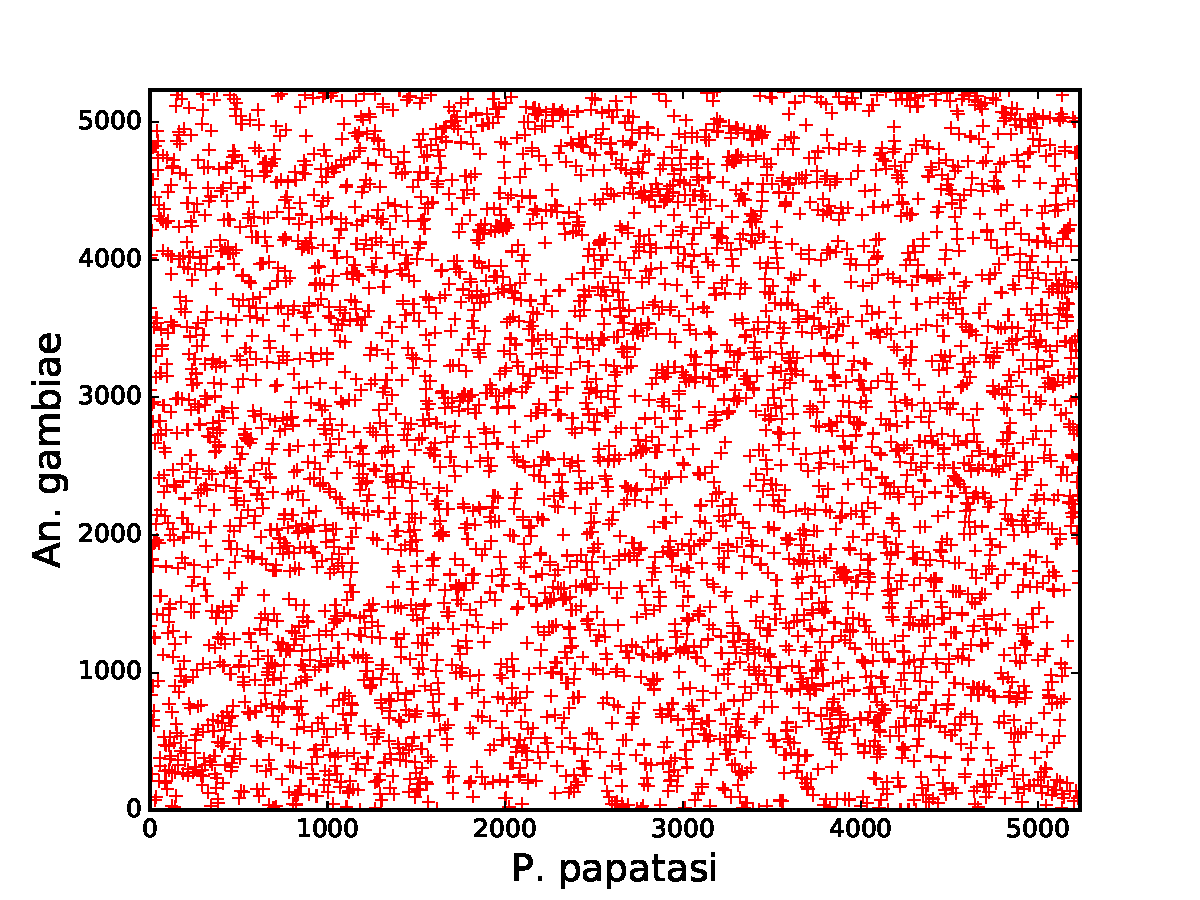
\includegraphics[width=\textwidth]{figures/synteny/papatasi_anopheles_plot}
    \caption{\emph{P. papatasi} vs. \emph{An. gambiae}}
    \label{fig:synteny-dotplots-papatasi-anopheles}
  \end{subfigure}
  ~
  \begin{subfigure}[b]{0.45\textwidth}
    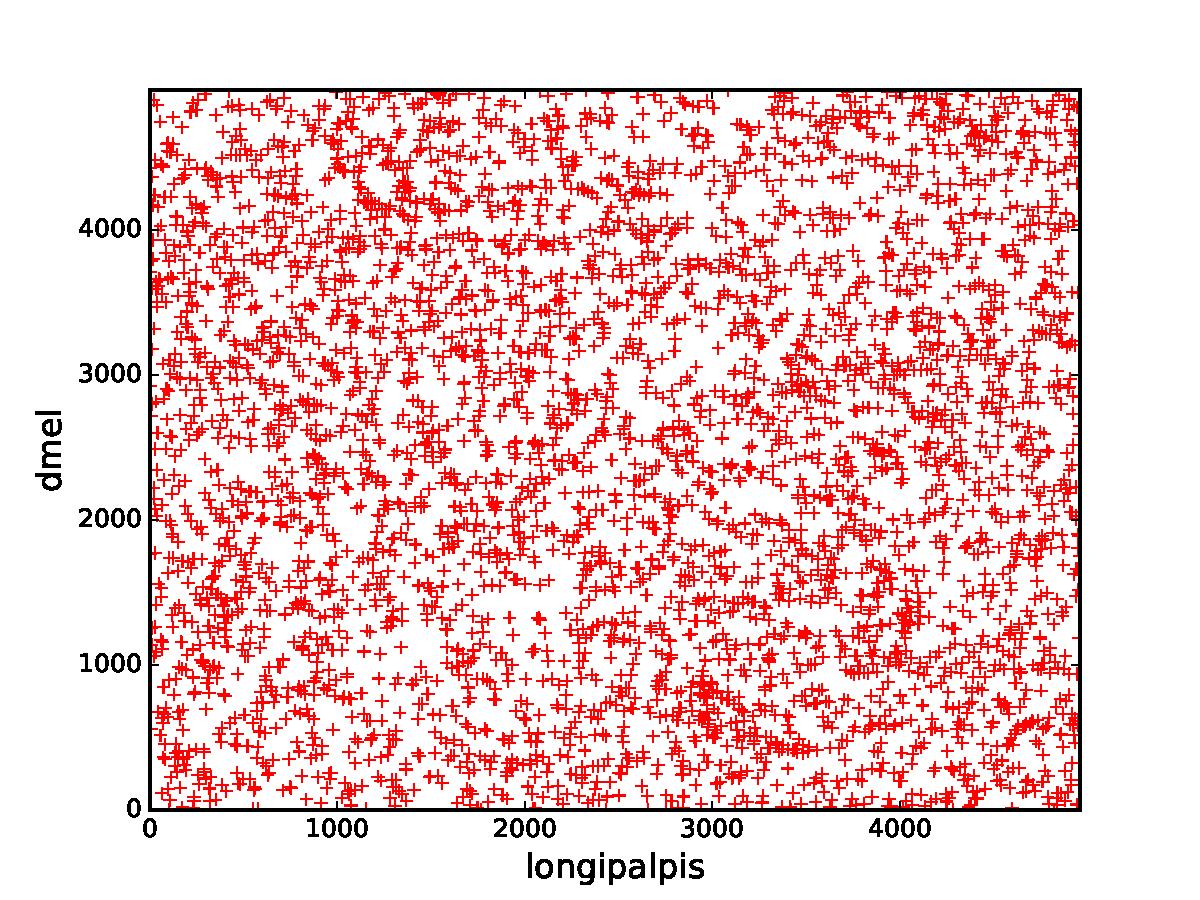
\includegraphics[width=\textwidth]{figures/synteny/longipalpis_dmel_plot}
    \caption{\emph{L. longipalpis} vs. \emph{D. melanogaster}}
    \label{fig:synteny-dotplots-longipalpis-dmel}
  \end{subfigure}
  ~
  \begin{subfigure}[b]{0.45\textwidth}
    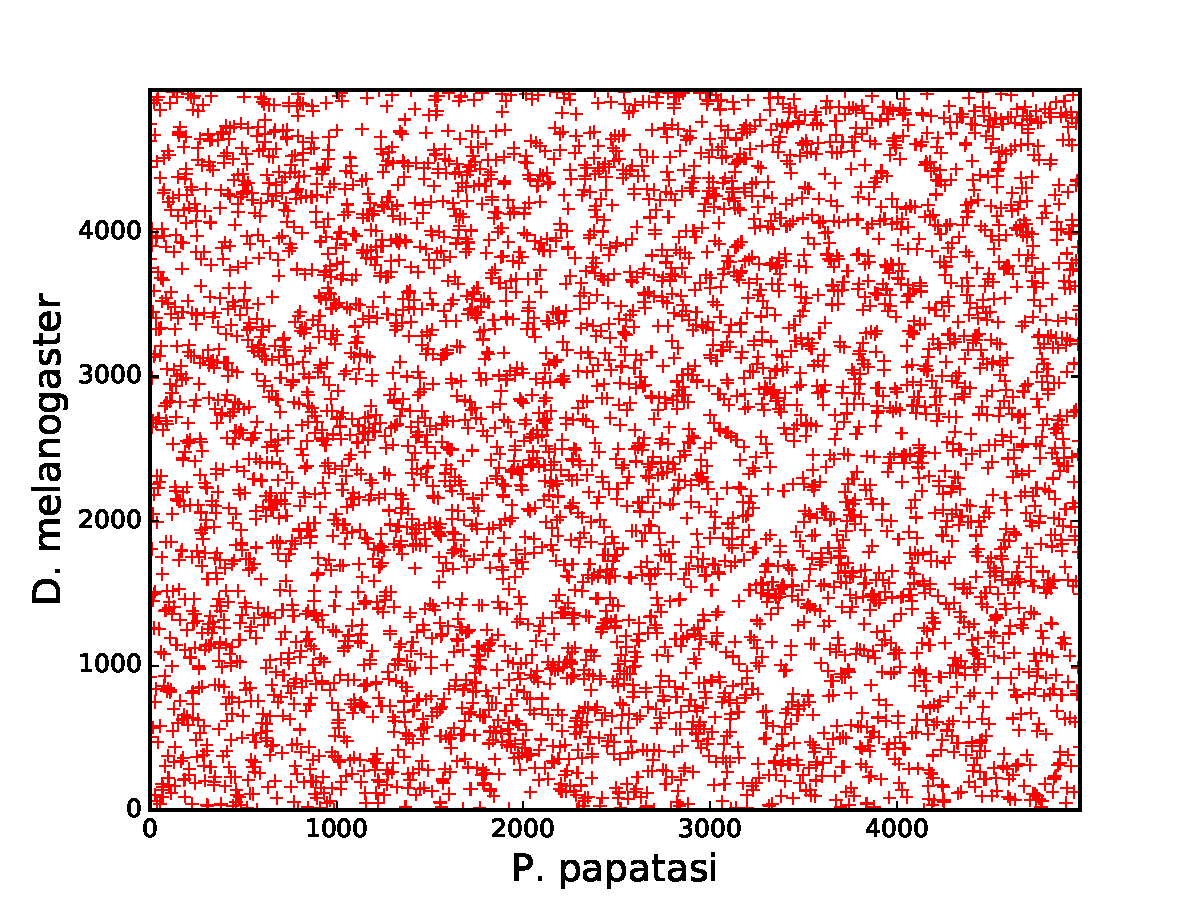
\includegraphics[width=\textwidth]{figures/synteny/papatasi_dmel_plot}
    \caption{\emph{P. papatasi} vs. \emph{D. melanogaster}}
    \label{fig:synteny-dotplots-papatasi-dmel}
  \end{subfigure}
  ~
  \begin{subfigure}[b]{0.45\textwidth}
    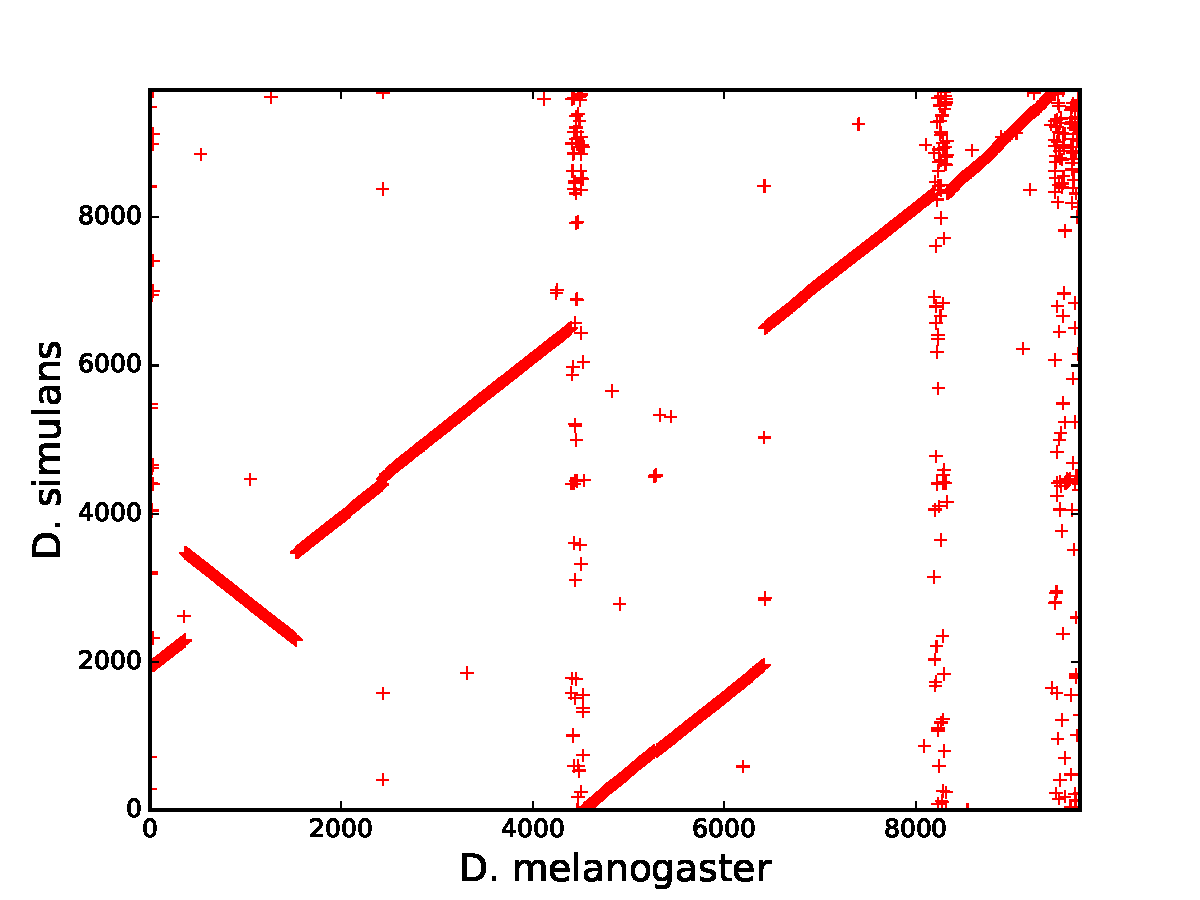
\includegraphics[width=\textwidth]{figures/synteny/dmel_dsim_plot}
    \caption{\emph{D. melanogaster} vs. \emph{D. simulans}}
    \label{fig:synteny-dotplots-drosophila}
  \end{subfigure}
  ~
  \begin{subfigure}[b]{0.45\textwidth}
    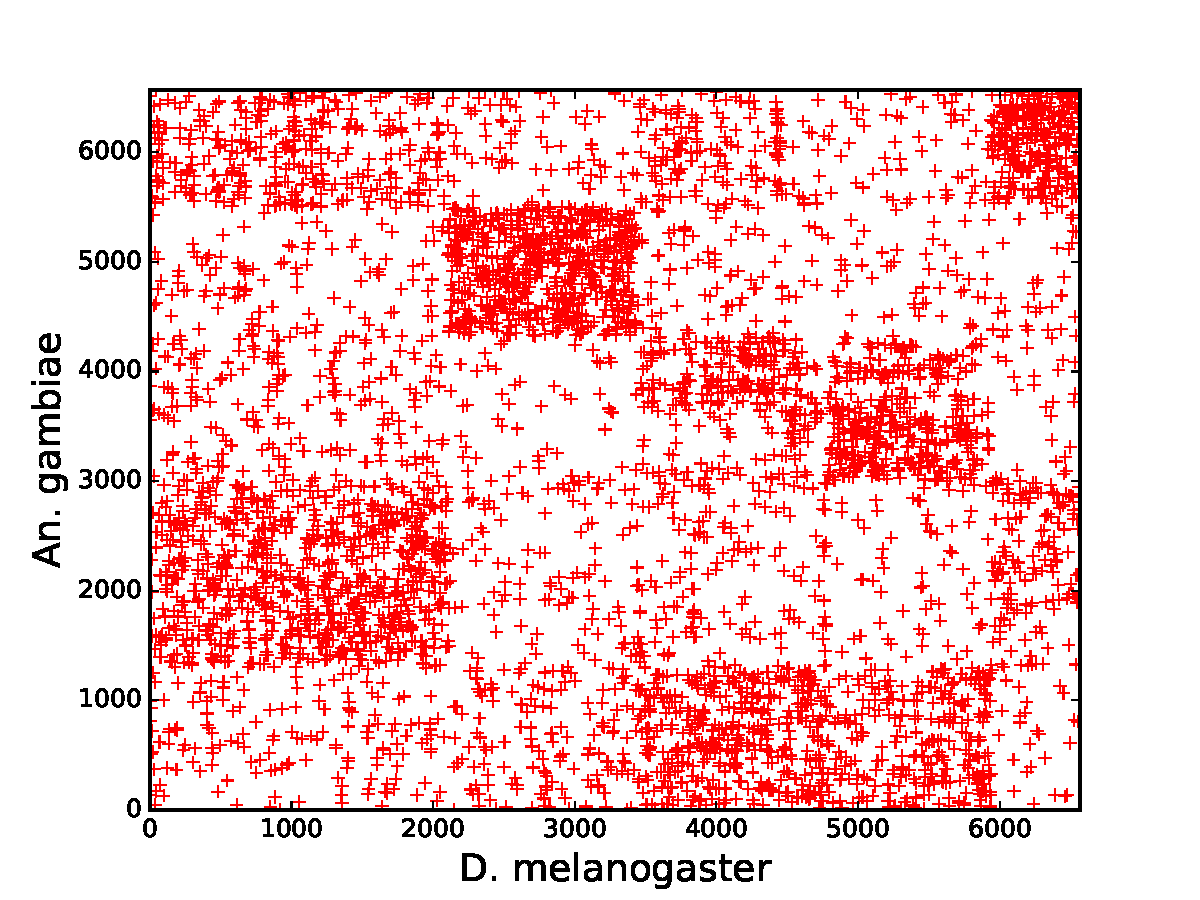
\includegraphics[width=\textwidth]{figures/synteny/dmel_anopheles_plot}
    \caption{\emph{A. gambiae} vs. \emph{D. melanogaster}}
    \label{fig:synteny-dotplots-anopheles-drosophila}
  \end{subfigure}
\label{fig:dot-plots}
\caption{Qualitative Analysis of Synteny}
\end{figure}

\begin{table}[H]
  \centering
  \begin{tabular}{c c c c c} \hline
    \emph{Species} & \emph{Count} & \emph{Average Size} & \emph{Median Size} & {Maximum Size} \\ \hline
    \emph{L. longipalpis} vs. \emph{An. gambiae} & 504 & 4.3 & 3 & 39 \\
    \emph{L. longipalpis} vs. \emph{P. papatasi} & 499 & 4.2 & 3 & 24 \\
    \emph{P. papatasi} vs. \emph{An. gambiae} & 307 & 4.3 & 3 & 21 \\
    \emph{D. melanogaster} vs. \emph{D. simulans} & 243 & 41.6 & 5 & 700 \\
    \emph{D. melanogaster} vs. \emph{An. gambiae} & 1037 & 2.5 & 2 & 10
  \end{tabular}
  \caption{Statistics including count and size (gene count) distributions for synteny blocks.}
  \label{tab:synteny-block-stats}
\end{table}

\subsection{Comparison of $d_N$/$d_S$ Distributions}
DNA base pairs are subject to random substitutions as organisms reproduce.  Substitutions in protein-coding open-reading frames can be divided into two types: silent mutations which do not affect the resulting amino acid sequences and non-silent mutations which do affect the resulting amino acid sequences and can affect gene function.  Silent mutations are assumed not to be under any sort of selection process, correlating with an organism's rate of evolutionary change.  Non-silent mutations are less likely to be passed on since they may impair the function of important genes; those that are inherited either do not impact gene function or are under selection pressure as an organism adapts.

dN/dS measures the ratio of the rate of substitutions at silent sites (dS), which are presumed neutral, to the rate of substitutions at non-silent sites (dN) \cite{Kryazhimskiy2008}. Genes with dN/dS $>$ 1 have non-silent substitions at a higher rate than the background rate of the organism's evolutionary change would suggest.  As such, these genes are assumed to be under selection pressure.  dN/dS is applied to orthologous genes from separate populations to identify genes which are likely associated with differences in populations' environments and ecological niches.

We analyzed dN/dS ratios between single-copy orthologs in pairwise comparisons of the sand flies \emph{L. longipalpis} and \emph{P. papatasi}, mosquito \emph{An. gambiae}, and fruit fly \emph{D. melanogaster}.  The distributions of dN/dS ratios are given in Figure~\ref{fig:dnds-distr}.  Except for the comparison between \emph{L. longipalpis} and \emph{P. papatasi}, the distributions are remarkedly similar.  The dN/dS distribution for \emph{L. longipalpis} vs \emph{P. papatasi} is skewed towards zero, indicating fewer non-silent substitutions than expected when the comparison to the other distributions.

\begin{figure}[H]
  \centering
  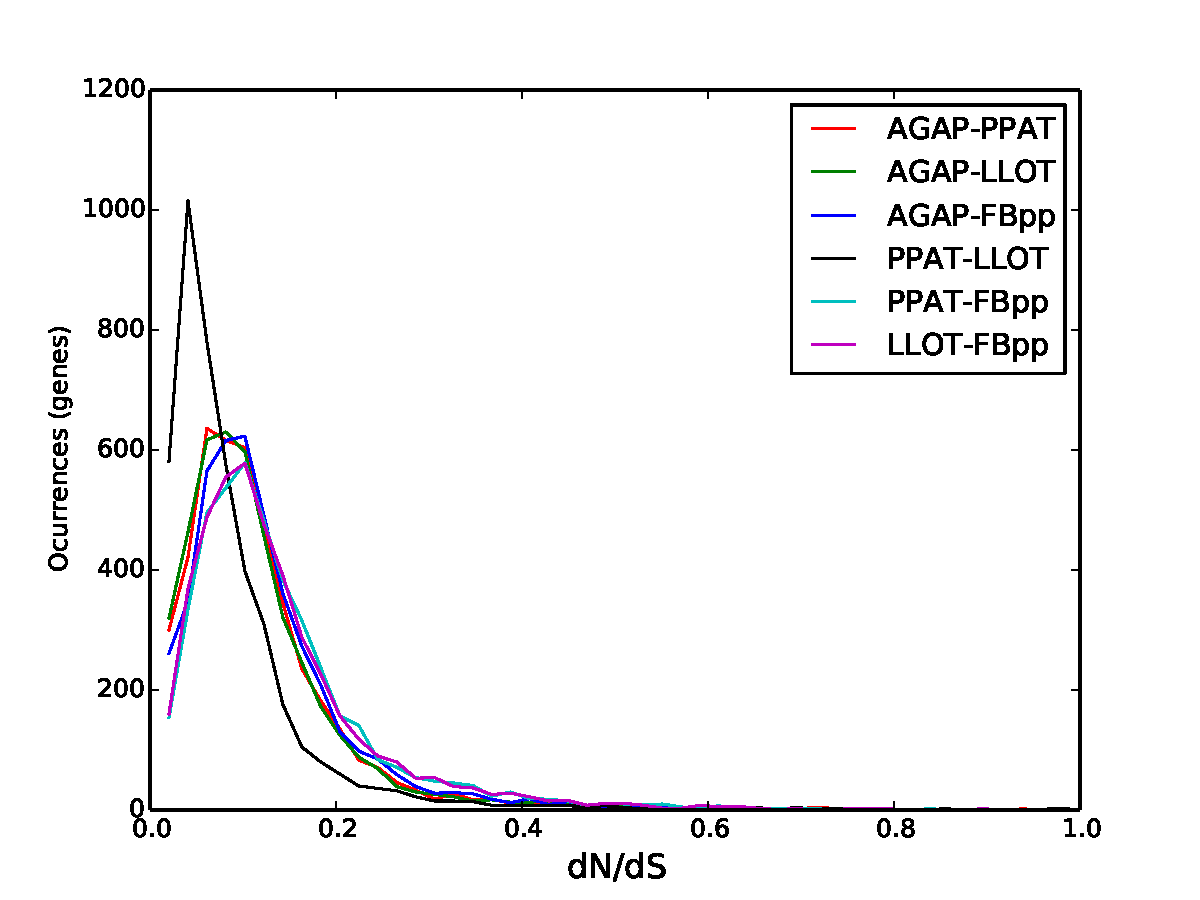
\includegraphics[width=0.75\textwidth]{figures/ka_ks/dN_dS}
  \caption{Distribution of dN/dS values}
  \label{fig:dnds-distr}
\end{figure}

\subsection{RNASeq Differential Gene Expression Analysis in Sugar-Fed, Blood-Fed, and Infected Blood-Fed \emph{L. longipalpis} Females}
RNASeq differental gene expression data was collected from \emph{L. longipalpis} females 6, 24, and 144 hours after being fed sugar, bloodmeals, and bloodmeals infected with the Leishmaniasis parasite, \emph{Leishmania major}.  We identified approximately 3,000 to 4,500 genes with statistically-significant differences in expression between blood-fed and sugar-fed females over the three time points (see Table~\ref{tab:stat-sig-genes}).  Fewer genes (about 250 to 670) had statistically-significantly differences in expression when compared between blood-fed and infected blood-fed females.

\begin{table}[H]
  \centering
  \begin{tabular}{c c c} \hline
  \emph{Time Point} & \emph{Blood Fed vs Sugar Fed} & \emph{Infected Blood Fed vs Blood Fed} \\ \hline
  6H & 3,111 & 271 \\ \hline
  24H & 4,120 & 658 \\ \hline
  144H & 4,571 & 290 \\ \hline
  \end{tabular}
  \caption{Number of Genes with Statistically-Significant Differential Expression}
  \label{tab:stat-sig-genes}
\end{table}

Comparison of GO-slim term distributions yielded little insight into differences in expression between the conditions due to the overwhelming number of genes with statistically-significant differences in expression.

As such, we focused on comparing expression of genes from families and pathways associated with immunity between blood fed and infected blood fed conditions.  The expression levels of Attacin-C (LLOTMP005408, IMD), LuloGalecC (LLOTMP007344, Galectins), and LuloDifA (LLOTMP002098, Toll) were increased under infected blood fed conditions for all time points.  MAP4K4 (MAPK), Caspar (LLOTMP002950, IMD), Rel (LLOTMP002098, IMD), and IAP2 (LLOTMP000523, IMD) had reduced expression levels under infected blood fed conditions for all time points.  MAP3K7 (MAPK), LuloToll3 (LLOTMP001885, Toll), LuloDifB (LLOTMP002097, Toll), CalcinuerinB (LLOTMP006044, IMD), COX (LLOTMP003300, IMD), and Prohenoloxidase (LLOTMP001742, IMD) had both increased and decreased in expression at various time points.

We also compared expression of genes involved with digestion from the peritrophin, chitin deacetylases, and chitinase families between blood fed and infected blood fed conditions. Increased expression of LuloPer1 (LLOTMP006497), LuloPer3a (LLOTMP002647), and LuloPer32 (LLOTMP00451) of the peritrophin familyand LlIDGF4 (LLOTMP004095) and chitinase like protein (LLOTMP006041) of the chitinase family was observed under infected blood fed conditions.  LuloPer3b (LLOTMP00490) and LuloPer2 (LLOTMP003676) of the peritropin family and LuloCDA1 (LLOTMP007910) of the chitin deacetylase family had both increased and decreased differences in expression between blood fed and infected blood fed conditions.

\subsection{Niemann Pick type C-like Genes}
A three-way comparison of synteny between \emph{An. gambiae}, \emph{L. longipalpis}, and \emph{P. papatasi} revealed a block of Niemann Pick type C2-like genes (Table~\ref{tab:synteny-three-way-npc2}). In insects, NPC genes are involved with sterol (e.g., cholesterol) homeostasis and biosynthesis of ecdysteroids, insect sex and moulting hormones. In humans, mutations in either of two Niemann Pick type C (NPC) genes, \emph{NPC1} and \emph{NPC2}, cause a fatal neurogenerative disorder associated with abnormal cholesterol accumulation in cells.  Previous work on NPC 2 in \emph{D. melanogaster} found that \emph{npc2a} and \emph{npc2b}, play a redundant role such that mutations in one have little discernable effect on biology; concurrent mutations in both genes lead to mortality and apoptotic neurodegeneration \cite{Huang2007}.  \emph{npc2e} and \emph{npc2a} have also been associated with the immune defiency (Imd) pathways in \emph{D. melanogaster} \cite{Shi2012}. Studies of NPC2-like genes in \emph{Ae. aegypti} have implicated ecdysteroids in a signaling cascade linking blood meal intake with vitellogenesis \cite{Sirot2011}.  Thus, the synteny of NPC2-like genes between \emph{An. gambiae}, \emph{L. longipalpis}, and \emph{P. papatasi}, may indicate similarity in sex, moulting, immunity, and feeding pathways between sand flies and mosquitoes.

We analyzed the differential gene expression in \emph{L. longipalpis} of the Niemann Pick type C2-like (NPC2) genes found to be in synteny between \emph{An. gambiae}, \emph{L. longipalpis}, and \emph{P. papatasi}.  Two genes (LLOTMP001859 and LLOTMP001861) presented statistically-significant differences in expression. Both genes had higher expression levels in blood fed or infected blood fed individuals 24 hours compared with sugar-fed individuals; by 144 hours elapsed, the genes' expression levels were significantly reduced compared to sugar-fed individuals.  The differences in expression levels between blood fed and sugar fed individuals seems to support the involvement of NPC2-like genes in a signaling cascade linking blood meal intake with vitellogenesis as observed in \emph{Ae. aegypti} \cite{Sirot2011}.

Whereas LLOTMP001861 presented little difference in expression between blood fed and infected blood fed individuals, LLOTMP001859 had significantly higher expression levels in infected blood fed individuals at 6 and 24 hours.  \emph{npc2e} and \emph{npc2a} have also been associated with the immune defiency (Imd) pathways in \emph{D. melanogaster} \cite{Shi2012}.  The differences in expression may indicate that LLOTMP001859 plays role in immune response to the leishmaniasis parasite.

\begin{table}[H]
  \centering
  \begin{tabular}{c c c l} \hline
    \emph{L. longipalpis} & \emph{P. papatasi} & \emph{An. gambiae} & \emph{Description} \\ \hline
    LLOTMP001853 & PPATMP007803 & AGAP002847 & Niemann-Pick like \\
    LLOTMP001854 & PPATMP007804 & AGAP002848 & Niemann-Pick like \\
    LLOTMP001855 & PPATMP007805 & AGAP002849 & Niemann-Pick like \\
    LLOTMP001857 & PPATMP007806 & AGAP002850 & Niemann-Pick like \\
    LLOTMP001858 & PPATMP007807 & AGAP002851 & Niemann-Pick like \\
    LLOTMP001859 & PPATMP007808 & AGAP002852 & Niemann-Pick like \\
    LLOTMP001861 & & AGAP002853 & Niemann-Pick like \\
    LLOTMP001863 & & AGAP002854 & Niemann-Pick like \\
    LLOTMP001864 & & AGAP002855 & Niemann-Pick like \\
    LLOTMP001865 & & AGAP002857 & Niemann-Pick like
    \end{tabular}
    \caption{Synteny block of Niemann-Pick like genes from \emph{L. longipalpis} vs. \emph{P. papatasi} vs. \emph{An. gambiae}.}
  \label{tab:synteny-three-way-npc2}
\end{table}

\subsection{Digestion-Related Genes}



\begin{table}[H]
  \centering
  \begin{tabular}{c c l} \hline
    \emph{L. longipalpis} & \emph{P. papatasi} & \emph{Description} \\ \hline
    LLOTMP006493 & PPATMP009348 & SCP-related protein \\
    LLOTMP006494 & PPATMP009349 & ribosomal protein S23 \\
    LLOTMP006495 & PPATMP009350 & Chitin-Binding Domain \\
    LLOTMP006496 & PPATMP009351 & Chitin-Binding Domain \\
    LLOTMP006497 & PPATMP009352 & Chitin-Binding Domain \\
    LLOTMP006498 & PPATMP009353 & Chitin-Binding Domain \\
    LLOTMP006499 & PPATMP009355 & Chitin-Binding Domain \\
    LLOTMP006500 & PPATMP009356 & Chitin-Binding Domain
  \end{tabular}
  \caption{Synteny block of peritrophic matrix-associated genes from \emph{L. longipalpis} vs. \emph{P. papatasi}.}
  \label{tab:synteny-llot-ppat-peritrophic}
\end{table}


\section{Discussion}
Comparative studies of synteny and gene order between insect genomes have indicated significant levels of genome shuffling, more so than observed in fish and humans \cite{Zdobnov2007}. A quantitative comparison of synteny and protein sequence identity using single-copy othologs from twelve insect genomes observed a linear relationship between the two metrics and the loss of all synteny

The sand fly genome assemblies are highly fragmented with genes distributed nearly uniformally across a large number of scaffolds (1,928 for \emph{L. longipalpis}, 4,350 for \emph{P. papatasi}).  Fragmentation is not unexpected given the high rates of genome shuffling observed in comparative analyses of insect genomes \cite{Zdobnov2007,Ranz2001}.  High rates of genome shuffling may limit the utility of well-assembled genomes as references in the assembly process, further complicating the assembly process.

Synteny analysis is dependent on the completeness of genome assemblies \cite{Heger2007}; the sizes of synteny blocks are naturally bounded by the size of the largest scaffolds.  The lack of significant macrosynteny between the sand flies and the \emph{An. gambiae} and \emph{D. melanogaster} reference genomes is limited by the high fragmention observed in the sand fly genome assembles.  However, as macrosynteny was also absent in the comparison of \emph{An. gambiae} and \emph{D. melanogaster}, whose genome assemblies are complete to the level of chromosomes, there simply may not be macrosynteny given the high rate of genome shuffling observed in insect genomes.

Microsynteny was, however, observed between the sand flies and the sand flies and \emph{An. gambiae}.  Annotation of the sand fly microsynteny blocks found common ``bookkeeping'' genes conserved across a large number of organisms such as genes associated with membrane transport, RNA regulation and synthesis, and intracellular processes \cite{Zdobnov2007}.  Genes associated with peritrophic matrices found primarily in insects were also found to be in microsynteny but are known to be well conserved across insects \textcolor{red}{cite}.  Microsynteny of such highly-conserved genes is expected.

Evolutionary changes at the level of indidividual genes was analyzed through comparing distributions of dN/dS ratios of single-copy orthologs.  The dN/dS distribution for \emph{L. longipalpis} vs \emph{P. papatasi} is skewed towards zero, indicating fewer non-silent substitutions than expected when the comparison to the distributions from pairwise comparisons with \emph{An. gambiae} and \emph{D. melanogaster}.  \textcolor{red}{closer evolutionarily?} The skew is more likely explained by issues with the \emph{L. longipalpis} vs \emph{P. papatasi} genomes assemblies than a biological cause.  In particular, the assemblies contain incomplete genes with only the most conserved regions present.  As such, regions of the sequences that likely diverged from their orthologous counterparts in other species are not present, biasing the dN/dS ratios towards zero.

Depletion of Caspar, a negative regulator of the immune deficiency (IMD) pathway, with RNA interference was previously shown to reduce population infection rates from 85\% to 45\% suggesting that the IMD pathway plays a role frustrates infection by \emph{L. major} \cite{Telleria2012}.  Our observation of reduced expression of Caspar under infected blood fed conditions warrants further analysis

Peritrophins

\section{Conclusion}





